\newpage	
\section{Teilversuch 1: Belastungsabhängigkeit zweier Spannungsquellen}

Leerlaufspannung vorher $U_0 = \SI{1.365(8)}{\volt}$ \\
Leerlaufspannung nachher $U_1 = \SI{1.354(8)}{\volt}$

Fehler bei der Strommessung $\Delta I = \pm 0,8\% \text{ Messwert} + 1 \text{ Digit}$ \\
Fehler bei der Spannungmessung $\Delta I = \pm 0,5\% \text{ Messwert} + 1 \text{ Digit}$
\begin{equation*}
	\begin{tabu}{l *{11}{l}}
		\toprule
		I/\si{\milli\ampere} & 10,6 & 13,4 & 16,2 & 19,1 & 21,9 & 24,8 & 27,5 & 30,6 & 33,1 & 35,9 & 38,7 \\
		\midrule
		U/\si{\volt} & 1,332 & 1,322 & 1,317 & 1,312 & 1,308 & 1,303 & 1,300 & 1,294 & 1,290 & 1,286 & 1,282 \\
		\bottomrule
	\end{tabu}
\end{equation*}
Die Daten wurden mit \gnuplot{} geplottet und es wurde eine Kurvenanpassung zur $U = mI + c$ durchgeführt. Die entsprechenden Fehler sind im \gnuplot{} direkt berechnet. Für die genaue Rechnung, siehe Appendix \ref{appdx:gnuplottv1}. 
\begin{figure}[H]
	\centering
	% GNUPLOT: LaTeX picture with Postscript
\begingroup
  \makeatletter
  \providecommand\color[2][]{%
    \GenericError{(gnuplot) \space\space\space\@spaces}{%
      Package color not loaded in conjunction with
      terminal option `colourtext'%
    }{See the gnuplot documentation for explanation.%
    }{Either use 'blacktext' in gnuplot or load the package
      color.sty in LaTeX.}%
    \renewcommand\color[2][]{}%
  }%
  \providecommand\includegraphics[2][]{%
    \GenericError{(gnuplot) \space\space\space\@spaces}{%
      Package graphicx or graphics not loaded%
    }{See the gnuplot documentation for explanation.%
    }{The gnuplot epslatex terminal needs graphicx.sty or graphics.sty.}%
    \renewcommand\includegraphics[2][]{}%
  }%
  \providecommand\rotatebox[2]{#2}%
  \@ifundefined{ifGPcolor}{%
    \newif\ifGPcolor
    \GPcolortrue
  }{}%
  \@ifundefined{ifGPblacktext}{%
    \newif\ifGPblacktext
    \GPblacktexttrue
  }{}%
  % define a \g@addto@macro without @ in the name:
  \let\gplgaddtomacro\g@addto@macro
  % define empty templates for all commands taking text:
  \gdef\gplbacktext{}%
  \gdef\gplfronttext{}%
  \makeatother
  \ifGPblacktext
    % no textcolor at all
    \def\colorrgb#1{}%
    \def\colorgray#1{}%
  \else
    % gray or color?
    \ifGPcolor
      \def\colorrgb#1{\color[rgb]{#1}}%
      \def\colorgray#1{\color[gray]{#1}}%
      \expandafter\def\csname LTw\endcsname{\color{white}}%
      \expandafter\def\csname LTb\endcsname{\color{black}}%
      \expandafter\def\csname LTa\endcsname{\color{black}}%
      \expandafter\def\csname LT0\endcsname{\color[rgb]{1,0,0}}%
      \expandafter\def\csname LT1\endcsname{\color[rgb]{0,1,0}}%
      \expandafter\def\csname LT2\endcsname{\color[rgb]{0,0,1}}%
      \expandafter\def\csname LT3\endcsname{\color[rgb]{1,0,1}}%
      \expandafter\def\csname LT4\endcsname{\color[rgb]{0,1,1}}%
      \expandafter\def\csname LT5\endcsname{\color[rgb]{1,1,0}}%
      \expandafter\def\csname LT6\endcsname{\color[rgb]{0,0,0}}%
      \expandafter\def\csname LT7\endcsname{\color[rgb]{1,0.3,0}}%
      \expandafter\def\csname LT8\endcsname{\color[rgb]{0.5,0.5,0.5}}%
    \else
      % gray
      \def\colorrgb#1{\color{black}}%
      \def\colorgray#1{\color[gray]{#1}}%
      \expandafter\def\csname LTw\endcsname{\color{white}}%
      \expandafter\def\csname LTb\endcsname{\color{black}}%
      \expandafter\def\csname LTa\endcsname{\color{black}}%
      \expandafter\def\csname LT0\endcsname{\color{black}}%
      \expandafter\def\csname LT1\endcsname{\color{black}}%
      \expandafter\def\csname LT2\endcsname{\color{black}}%
      \expandafter\def\csname LT3\endcsname{\color{black}}%
      \expandafter\def\csname LT4\endcsname{\color{black}}%
      \expandafter\def\csname LT5\endcsname{\color{black}}%
      \expandafter\def\csname LT6\endcsname{\color{black}}%
      \expandafter\def\csname LT7\endcsname{\color{black}}%
      \expandafter\def\csname LT8\endcsname{\color{black}}%
    \fi
  \fi
    \setlength{\unitlength}{0.0500bp}%
    \ifx\gptboxheight\undefined%
      \newlength{\gptboxheight}%
      \newlength{\gptboxwidth}%
      \newsavebox{\gptboxtext}%
    \fi%
    \setlength{\fboxrule}{0.5pt}%
    \setlength{\fboxsep}{1pt}%
\begin{picture}(8640.00,5760.00)%
    \gplgaddtomacro\gplbacktext{%
      \csname LTb\endcsname%%
      \put(682,704){\makebox(0,0)[r]{\strut{}$25$}}%
      \put(682,1192){\makebox(0,0)[r]{\strut{}$26$}}%
      \put(682,1681){\makebox(0,0)[r]{\strut{}$27$}}%
      \put(682,2169){\makebox(0,0)[r]{\strut{}$28$}}%
      \put(682,2657){\makebox(0,0)[r]{\strut{}$29$}}%
      \put(682,3146){\makebox(0,0)[r]{\strut{}$30$}}%
      \put(682,3634){\makebox(0,0)[r]{\strut{}$31$}}%
      \put(682,4122){\makebox(0,0)[r]{\strut{}$32$}}%
      \put(682,4611){\makebox(0,0)[r]{\strut{}$33$}}%
      \put(682,5099){\makebox(0,0)[r]{\strut{}$34$}}%
      \put(814,484){\makebox(0,0){\strut{}$-100$}}%
      \put(1489,484){\makebox(0,0){\strut{}$0$}}%
      \put(2165,484){\makebox(0,0){\strut{}$100$}}%
      \put(2840,484){\makebox(0,0){\strut{}$200$}}%
      \put(3515,484){\makebox(0,0){\strut{}$300$}}%
      \put(4191,484){\makebox(0,0){\strut{}$400$}}%
      \put(4866,484){\makebox(0,0){\strut{}$500$}}%
      \put(5542,484){\makebox(0,0){\strut{}$600$}}%
      \put(6217,484){\makebox(0,0){\strut{}$700$}}%
      \put(6892,484){\makebox(0,0){\strut{}$800$}}%
      \put(7568,484){\makebox(0,0){\strut{}$900$}}%
      \put(8243,484){\makebox(0,0){\strut{}$1000$}}%
    }%
    \gplgaddtomacro\gplfronttext{%
      \csname LTb\endcsname%%
      \put(209,2901){\rotatebox{-270}{\makebox(0,0){\strut{}Temperatur $\theta$ ($\si{\celsius}$)}}}%
      \put(4528,154){\makebox(0,0){\strut{}Zeit $t$ ($\si{\second}$)}}%
      \csname LTb\endcsname%%
      \put(946,4893){\makebox(0,0)[l]{\strut{}$0,00832t + 25,66397$}}%
      \csname LTb\endcsname%%
      \put(946,4607){\makebox(0,0)[l]{\strut{}Messpunkte}}%
      \csname LTb\endcsname%%
      \put(4528,5429){\makebox(0,0){\strut{}Erwärmung von Wasser im Kalorimeter}}%
    }%
    \gplbacktext
    \put(0,0){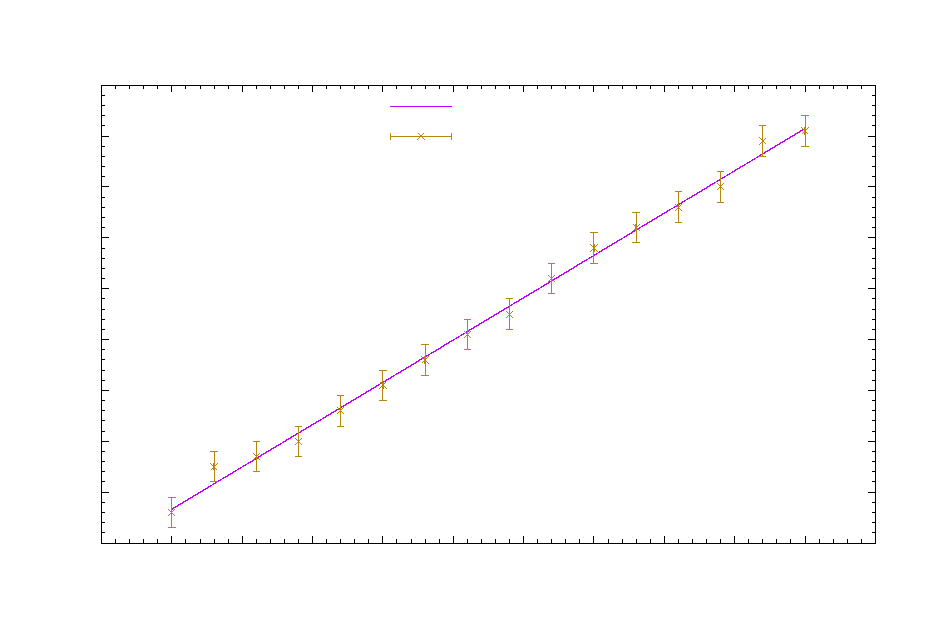
\includegraphics[width={432.00bp},height={288.00bp}]{tv1-plot}}%
    \gplfronttext
  \end{picture}%
\endgroup

	\caption{\centering Belastungsabhängigkeit einer galvanischen Zelle \captionbr $\chi^2_{\text{red}} = \num{0.0525026} \implies$ Gute Anpassung}
	\label{fig:tvone-plot}
	\vspace{-1em}
\end{figure}
Als Endergebnis erhalten wir:
\begin{equation*}
	\begin{tabu}{lll}
		\toprule
		\text{Variable} & \text{Wert} & \text{Gerundet} \\
		\midrule
		m & \SI{-1.67333(5845)e-3}{\kilo\ohm} & \SI{-1.67(6)}{\ohm}\\
		c & \SI{1.34552(155)}{\volt} & \SI{1.3455(16)}{\volt} \\
		\bottomrule
	\end{tabu}
\end{equation*}
Aus Gleichung (7) der Anleitung entspricht die Steigung $m$ den Innenwiderstand $R_i$, also ist der Innenwiderstand $R_i = \SI{1.67}{\ohm}$. 

Die extraploierte Leerlaufspannung ist gegeben durch $U_q = \SI{1.3455(16)}{\volt}$, was kleiner als die gemessene Leerlaufspannung ist. Das ist vermütlich wegen der nicht vernachlässigbaren Widerstand des als Amperemeter benutzten Multimeters.

Für das Netzgerät ergibt sich das folgende Verhältnis:
\begin{figure}[H]
	\centering
	% GNUPLOT: LaTeX picture with Postscript
\begingroup
  \makeatletter
  \providecommand\color[2][]{%
    \GenericError{(gnuplot) \space\space\space\@spaces}{%
      Package color not loaded in conjunction with
      terminal option `colourtext'%
    }{See the gnuplot documentation for explanation.%
    }{Either use 'blacktext' in gnuplot or load the package
      color.sty in LaTeX.}%
    \renewcommand\color[2][]{}%
  }%
  \providecommand\includegraphics[2][]{%
    \GenericError{(gnuplot) \space\space\space\@spaces}{%
      Package graphicx or graphics not loaded%
    }{See the gnuplot documentation for explanation.%
    }{The gnuplot epslatex terminal needs graphicx.sty or graphics.sty.}%
    \renewcommand\includegraphics[2][]{}%
  }%
  \providecommand\rotatebox[2]{#2}%
  \@ifundefined{ifGPcolor}{%
    \newif\ifGPcolor
    \GPcolortrue
  }{}%
  \@ifundefined{ifGPblacktext}{%
    \newif\ifGPblacktext
    \GPblacktexttrue
  }{}%
  % define a \g@addto@macro without @ in the name:
  \let\gplgaddtomacro\g@addto@macro
  % define empty templates for all commands taking text:
  \gdef\gplbacktext{}%
  \gdef\gplfronttext{}%
  \makeatother
  \ifGPblacktext
    % no textcolor at all
    \def\colorrgb#1{}%
    \def\colorgray#1{}%
  \else
    % gray or color?
    \ifGPcolor
      \def\colorrgb#1{\color[rgb]{#1}}%
      \def\colorgray#1{\color[gray]{#1}}%
      \expandafter\def\csname LTw\endcsname{\color{white}}%
      \expandafter\def\csname LTb\endcsname{\color{black}}%
      \expandafter\def\csname LTa\endcsname{\color{black}}%
      \expandafter\def\csname LT0\endcsname{\color[rgb]{1,0,0}}%
      \expandafter\def\csname LT1\endcsname{\color[rgb]{0,1,0}}%
      \expandafter\def\csname LT2\endcsname{\color[rgb]{0,0,1}}%
      \expandafter\def\csname LT3\endcsname{\color[rgb]{1,0,1}}%
      \expandafter\def\csname LT4\endcsname{\color[rgb]{0,1,1}}%
      \expandafter\def\csname LT5\endcsname{\color[rgb]{1,1,0}}%
      \expandafter\def\csname LT6\endcsname{\color[rgb]{0,0,0}}%
      \expandafter\def\csname LT7\endcsname{\color[rgb]{1,0.3,0}}%
      \expandafter\def\csname LT8\endcsname{\color[rgb]{0.5,0.5,0.5}}%
    \else
      % gray
      \def\colorrgb#1{\color{black}}%
      \def\colorgray#1{\color[gray]{#1}}%
      \expandafter\def\csname LTw\endcsname{\color{white}}%
      \expandafter\def\csname LTb\endcsname{\color{black}}%
      \expandafter\def\csname LTa\endcsname{\color{black}}%
      \expandafter\def\csname LT0\endcsname{\color{black}}%
      \expandafter\def\csname LT1\endcsname{\color{black}}%
      \expandafter\def\csname LT2\endcsname{\color{black}}%
      \expandafter\def\csname LT3\endcsname{\color{black}}%
      \expandafter\def\csname LT4\endcsname{\color{black}}%
      \expandafter\def\csname LT5\endcsname{\color{black}}%
      \expandafter\def\csname LT6\endcsname{\color{black}}%
      \expandafter\def\csname LT7\endcsname{\color{black}}%
      \expandafter\def\csname LT8\endcsname{\color{black}}%
    \fi
  \fi
    \setlength{\unitlength}{0.0500bp}%
    \ifx\gptboxheight\undefined%
      \newlength{\gptboxheight}%
      \newlength{\gptboxwidth}%
      \newsavebox{\gptboxtext}%
    \fi%
    \setlength{\fboxrule}{0.5pt}%
    \setlength{\fboxsep}{1pt}%
\begin{picture}(8640.00,5760.00)%
    \gplgaddtomacro\gplbacktext{%
      \csname LTb\endcsname%%
      \put(946,704){\makebox(0,0)[r]{\strut{}$7,5$}}%
      \put(946,1437){\makebox(0,0)[r]{\strut{}$8$}}%
      \put(946,2169){\makebox(0,0)[r]{\strut{}$8,5$}}%
      \put(946,2902){\makebox(0,0)[r]{\strut{}$9$}}%
      \put(946,3634){\makebox(0,0)[r]{\strut{}$9,5$}}%
      \put(946,4367){\makebox(0,0)[r]{\strut{}$10$}}%
      \put(946,5099){\makebox(0,0)[r]{\strut{}$10,5$}}%
      \put(1078,484){\makebox(0,0){\strut{}$0$}}%
      \put(1974,484){\makebox(0,0){\strut{}$200$}}%
      \put(2869,484){\makebox(0,0){\strut{}$400$}}%
      \put(3765,484){\makebox(0,0){\strut{}$600$}}%
      \put(4661,484){\makebox(0,0){\strut{}$800$}}%
      \put(5556,484){\makebox(0,0){\strut{}$1000$}}%
      \put(6452,484){\makebox(0,0){\strut{}$1200$}}%
      \put(7347,484){\makebox(0,0){\strut{}$1400$}}%
      \put(8243,484){\makebox(0,0){\strut{}$1600$}}%
    }%
    \gplgaddtomacro\gplfronttext{%
      \csname LTb\endcsname%%
      \put(209,2901){\rotatebox{-270}{\makebox(0,0){\strut{}Spannung $U$ ($\si{\volt}$)}}}%
      \put(4660,154){\makebox(0,0){\strut{}Belastungsstrom $I$ ($\si{\milli\ampere}$)}}%
      \csname LTb\endcsname%%
      \put(7256,4893){\makebox(0,0)[r]{\strut{}Messpunkte}}%
      \csname LTb\endcsname%%
      \put(7256,4607){\makebox(0,0)[r]{\strut{}glatter Spline durch Daten}}%
      \csname LTb\endcsname%%
      \put(4660,5429){\makebox(0,0){\strut{}Klemmenspannung eines Netzgeräts gegen den Belastungsstrom}}%
    }%
    \gplbacktext
    \put(0,0){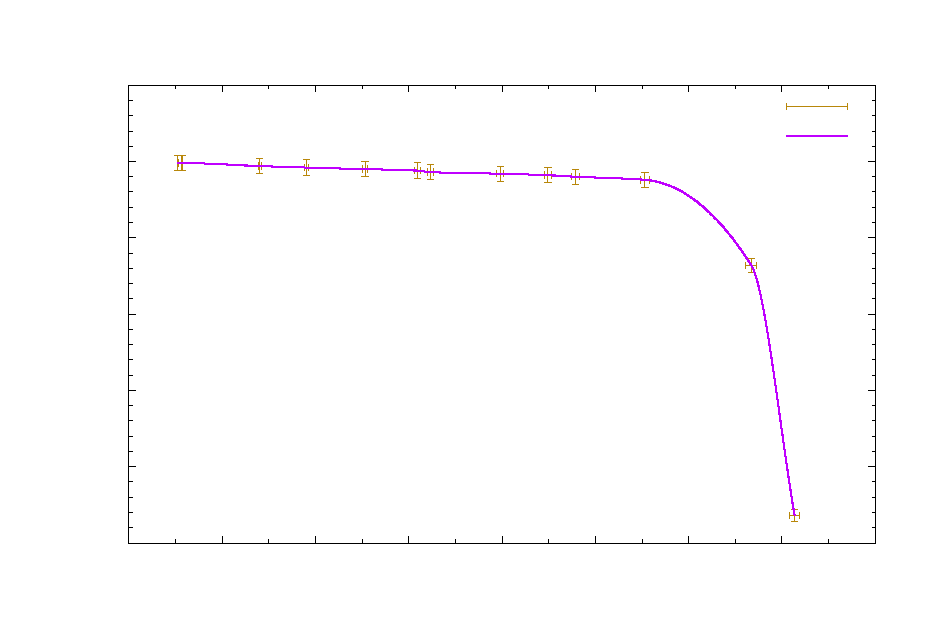
\includegraphics[width={432.00bp},height={288.00bp}]{tv1-ng-plot}}%
    \gplfronttext
  \end{picture}%
\endgroup

	\caption{\centering Belastungsabhängigkeit eines Netzgerät}
	\label{fig:tvone-ng-plot}
	\vspace{-1em}
\end{figure}
Für einen Belastungsstrom unterhalb ca. $\SI{1.1}{\ampere}$ ist die Spannung relativ stabil, was bei der galvanischen Zelle nicht der Fall ist. Danach gibt es eine deutliche Sprung bei ca. $\SI{1.3}{\ampere}$ und die nimmt stetig Spannung stetig ab. 

Mit dem Netzgerät gibt es also eine Belastungsgrenze, nachdem das Netzgerät keine stabile Spannung behalten kann. Mit der galvanische Zelle gibt es überhaupt keine stabile Spannung und wird je nach Belastungsstrom unterschiedliche Spannung liefern. 

Es gibt diese Unterschied, weil das Netzgerät von elektronischen Mitteln geregelt ist und theoretisch beliebig viel Strom vom Stromnetz ziehen kann (im Praxis gibt es eine obere Schranke), um die Ausgangsspannung aufrechtszuerhalten. Das Netzgerät ist also eine stabilierte Spannungsquelle. Bei der galvanische Zelle gibt es aber nur die Spannung aus dem gespeicherten chemischen Potential, deshalb sinkt die Spannung mit steigendem Strom. 